\documentclass[11pt, a4paper, spanish]{article}

%%%%%%%%%% COMIENZO DEL PREAMBULO %%%%%%%%%%

%Info sobre este documento
\author{Martin Cammi}
\title{Trabajo Pr'actico de Ingenier'ia del software I}

%\usepackage{infostyle}                                                  % provee un look & feel similar a un documento Word
\usepackage[top=2.5cm, bottom=2.5cm, left=2.5cm, right=2.5cm]{geometry}  % m�rgenes
\usepackage[ansinew]{inputenc}                                           % permite que los acentos del estilo ����� salgan joya
\usepackage[spanish, activeacute]{babel}                                 % idioma espa�ol, acentos f�ciles y deletreo de palabras
\usepackage{indentfirst}                                                 % permite indentar un parrafo a mano
\usepackage{caratula}                                                    % incluye caratula est�ndar
\usepackage{graphicx}                                                    % permite insertar gr�ficos
\usepackage{color}                                                       % permite el uso de colores en el documento
\usepackage[pdfcreator={TexLive!, LaTeX2e con TeXnicCenter y la inteligencia de Jonathan ;-)},
			pdfauthor={Grupo 1"},
			pdftitle={Ingenieria del Software - Trabajo practico: sistema de software CentralMarket},
			pdfsubject={Trabajo Practico de Modelado de dominio},
			pdfkeywords={Contenidos, proveedor, bajo demanda},
			pdfstartview=FitH,            % Fits the width of the page to the window
			bookmarksnumbered,            % los bookmarks numerados se ven mejor...
			colorlinks,                   % links con bellos colores
			linkcolor=magenta]            % permite cambiar el color de los links
			{hyperref}                                                         % Permite jugar con algunas cosas que aparecer�n en el PDF final

%\selectlanguage{spanish}

\linespread{1.3}                    % interlineado equivalente al 1.5 l�neas de Word...
\pagestyle{myheadings}              %encabezado personalizable con \markboth{}{}
\markboth{}{Ingenieria del Software - TP de Modelado de Objetivos}
\headsep = 30pt                     % separaci�n entre encabezado y comienzo del p�rrafo

%\addtolength{\oddsidemargin}{-2cm}	% configuracion IDEAL!!!
%\addtolength{\textwidth}{4cm}
%\addtolength{\textheight}{2cm}

% macro 'todo' para To-Do's
\def\todo#1{\textcolor{red}{#1}}

% Macro 'borde' para un texto con borde
\newsavebox{\fmbox}
\newenvironment{borde}[1]
{\begin{lrbox}{\fmbox}\begin{minipage}{#1}}
{\end{minipage}\end{lrbox}\fbox{\usebox{\fmbox}}\\[10pt]}

%%%%%%%%%% FIN DEL PREAMBULO %%%%%%%%%%

\begin{document}

\materia{Ingenier\'ia de Software I}
\submateria{Primer Cuatrimestre de 2012}
\titulo{Trabajo pr\'actico 1}
\subtitulo{An\'alisis preliminar de un sistema de software para CentralMarket}
\grupo{Grupo 1}

\integrante{Abreg\'u, Angel}{082/09}{angelj\_a@hotmail.com}
\integrante{Cammi, Mart\'in}{676/02}{martincammi@gmail.com}
\integrante{De Sousa, Mariano}{389/08}{marian\_sabianaa@hotmail.com}
\integrante{M�ndez, Gonz\'alo}{843/04}{gemm83@hotmail.com}
\integrante{Raffo, Diego}{423/08}{enanodr@hotmail.com}


\maketitle

\thispagestyle{empty}

\tableofcontents

\newpage

% Conviene poner las secciones como diferentes archivos,
% sobre todo cuando se trabaja en equipo.
% Es m�s f�cil para sincronizar mediante control de versiones.
%\input{Introducci�n}


% BEGIN Ejemplos de uso

	%\section{Una secci�n}
	%\label{sec:unaSeccion}
	%Hola! Soy una Secci�n
	%	\subsection{Una subsecci�n}
	%		Y yo soy una subsecci�n!!!
	%		\subsubsection{Una subsubsecci�n}
	%			Y yo soy una sub-subsecci�n!!!
	%			\paragraph{Un p�rrafo\\}
	%				Y yo soy un p�rrafo, porque no hay mas sub-sub-sub-subsecciones!!!

	%\section{Otra secci�n}
	%	Como pudimos ver en la secci�n \ref{sec:unaSeccion}, esto es una demo de una referencia a una secci�n.
	
	%	Tambi�n podemos hacer referencia a la p�gina de la secci�n:\\[10pt]
	
		% Ejemplo de uso de un borde (falta pulir para que no tire un warning!)
	%	\begin{borde}{0.98\textwidth}
	%		En la p�gina \pageref{sec:unaSeccion}, hay una secci�n pilla...
	%	\end{borde}

% END Ejemplos de uso


\section{Propuesta de servicios}
\label{sec:Propuesta de servicios}

\subsection{Introducci\'on}
	Proporcionar la mayor cantidad de informaci\'on posible respecto de como nuestra propuesta ayudar� a cumplir con los objetivos planteados.

	La propuesta siguiente propuesta consiste en un modelo de objetivos que intenta concentrar las necesidades descriptas por el cliente.

	Nuestro objetivo principal es el de 
	

	

\subsection{Diagramas de Objetivos}



\section{Alcance de la aplicaci\'on}

	\begin{center}
		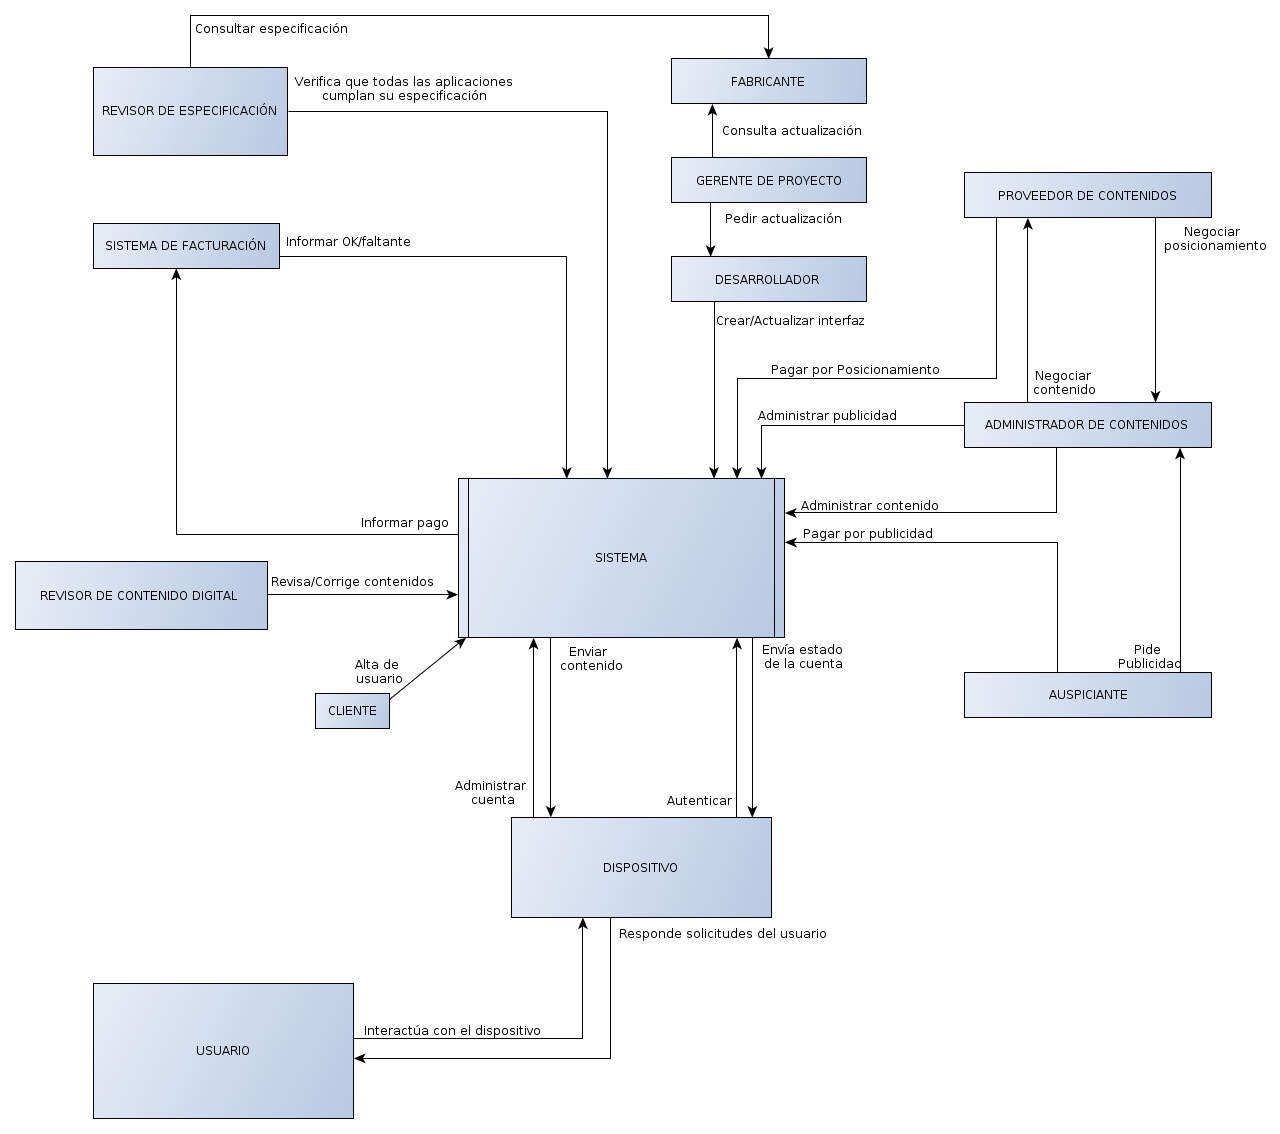
\includegraphics[scale=0.35]{graficos/DiagramaContexto.png}
	\end{center}

	Gr\'afico de Modelo de Jackson
	Explicar la relaci\'on del sistema con los usuarios hardware y otros sistemas.



	Ac� van los diagramas de objetivis

\section{Escenarios informales y ejemplos}
	
	Colocar texto de escenarios y ejemplos.

\end{document}
